\documentclass{article}
\usepackage[utf8]{inputenc}
\usepackage[portuguese]{babel}
\usepackage[margin=2.5cm]{geometry}
\setlength{\parskip}{1mm}
\setlength{\parindent}{10mm}
\linespread{1.2}
\usepackage[usenames,dvipsnames,svgnames,table]{xcolor}
\usepackage{fancyhdr}
\usepackage[symbol]{footmisc}
\usepackage{amsfonts,amsmath,amssymb,amsthm}
\newtheorem{thm}{Teorema}[]
\usepackage{array,caption,graphicx}
\usepackage[shortlabels]{enumitem}
\usepackage{verbatim}
\usepackage{listings}
\usepackage{float}
\usepackage{graphicx}
\graphicspath{ {./images/} }
\definecolor{codegreen}{rgb}{0,0.6,0}
\definecolor{codegray}{rgb}{0.5,0.5,0.5}
\definecolor{codepurple}{rgb}{0.58,0,0.82}
\definecolor{backcolour}{rgb}{0.95,0.95,0.92}
\lstdefinestyle{mystyle}{
  backgroundcolor=\color{backcolour},   commentstyle=\color{codegreen},
  keywordstyle=\color{magenta},
  numberstyle=\tiny\color{codegray},
  stringstyle=\color{codepurple},
  basicstyle=\footnotesize,
  breakatwhitespace=false,
  breaklines=true,
  captionpos=b,
  keepspaces=true,
  numbers=left,
  numbersep=5pt,
  showspaces=false,
  showstringspaces=false,
  showtabs=false,
  tabsize=2
}
\renewcommand{\thefootnote}{\arabic{footnote}}
\lstset{style=mystyle}


\title{\textbf{Análise Numérica\\Relatório 2 - Determinação de Raízes}}
\author{\textbf{Grupo 29}\\[4mm]José Dias\\Luís Pinto\\Samuel Neves\\Bárbara Gonçalves\\}
\date{27 de Março de 2019}
\begin{document}
\maketitle
\clearpage
\pagestyle{fancy}
\fancyhf{}
\setlength{\headheight}{30pt}
\rhead{Relatório nº2}
\lhead{\textbf{Grupo 29}}
\setlength{\footskip}{15pt}
\rfoot{\thepage}
\section{Introdução}
\hspace{6mm}Com este trabalho pretendemos determinar raízes de uma dada função usando o método de Newton e o método iterativo simples com um erro inferior a um dado $\epsilon$. Dito isto, alguns pontos a ter em consideração quanto ao mesmo:
\begin{enumerate}
  \item{A linguagem utilizada foi \textit{Python} e \textit{wxMaxima}, portanto, os cálculos foram feitos em dupla precisão.}
  \item{Para a auxiliar a resposta ao problema em questão serão usados alguns dos seguintes métodos:}
  \begin{enumerate}
    \item[\textbullet]{Resolução Teórica;}
    \item[\textbullet]{Código do programa;}
    \item[\textbullet]{Gráficos;}
    \item[\textbullet]{Tabelas;}
    \item[\textbullet]{Comentários.}
  \end{enumerate}
  \item{A função $F$ referida em todos os exercícios é $F(x)=sin(10x)-x-0.1$ que é contínua em todo o seu domínio, pois resulta da soma e composição de funções contínuas.}
\end{enumerate}
\section*{Exercício 1.}
\subsection*{Alínea a)}
\begin{lstlisting}[language=Python]
from math import *
def F(x): #Funcao dada
    return sin(10*x)-x-0.1
def dfdx(x):  #Derivada da funcao dada
    return 10*cos(10*x)-1
def suc1(n,x0): '''n-esimo termo da sucessao x_n'''
    x = x0
    for i in range(n):
        x = -F(x)/dfdx(x)+x
    return x
def Ex1():
    x0 = float(input('Indique o valor inicial, x0: '))
    epsilon = input('Indique o erro que pretende estimar a sua solucao: ').split('*')
    if epsilon[0]=='10':
        epsilon = float(int(epsilon[0])**int(epsilon[2]))
    else:
        epsilon = float(int(epsilon[0])*10**int((epsilon[3])))
    count = 0
    erro = abs(x0-(-F(x0)/dfdx(x0)+x0))
    while erro > epsilon:
        x1 = x0
        x0 = suc1(1,x0)
        erro = abs(x0-x1)
        count+=1
        if count>100000:
          print('Numero de iteracoes excedida.', 'Erro =',erro, 'x0 =',x0)
          return('void')
    print('Foram precisas %d iteracoes e o valor obtido foi'% (count),x0, "erro absoluto estimado: ",erro)
\end{lstlisting}
\subsection*{Alínea b)}
\textbf{Gráfico de F(x):}\\
\begin{minipage}{0.6\textwidth}
\begin{figure}[H]
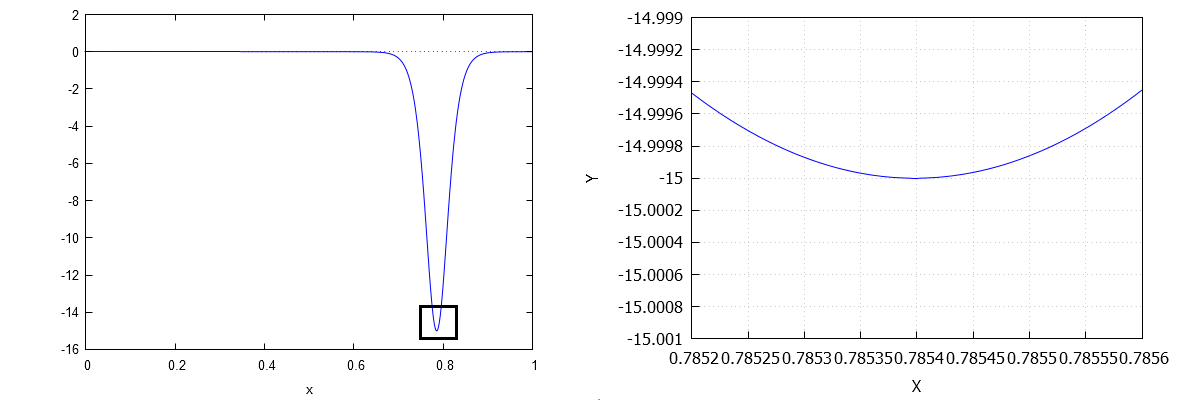
\includegraphics[scale=0.4]{./figure1.png}
\caption{Gráfico da função $y=F(x)$}
\end{figure}
\end{minipage}
\begin{minipage}{0.3\textwidth}
\textbf{Separação das Raízes:}\\[5mm]
\begin{tabular}{c|c}
    $ x $ & $F(x)$\\
    \hline
    -1  & $ \approx 1.444>0 $\\
    -0.75 & $\approx-0.288<0$\\
    -0.5 & $\approx1.359>0$\\
    -0.25 & $\approx-0.448$\\
    0.1 & $\approx0.641>0$\\
    0.5 & $\approx-1.559<0$ \\
    0.75 & $\approx0.088>0$\\
    1 & $\approx-1.641<0 $\\
\end{tabular}
\end{minipage}\\[5mm]
\textbf{Análise do gráfico e tabela:}\par
Analisando o gráfico da função F(x) verifica-se que tem 7 raízes e, com auxílio da \textit{Fig.1} obtém-se a separação das raízes nos seguintes intervalos:
  \begin{enumerate}
    \item $[-1,-0.75]$
    \item $[-0.75,-0.5]$
    \item $[-0.5,-0.25]$
    \item $[-0.25,0.1]$
    \item $[0.1,0.5]$
    \item $[0.5,0.75]$
    \item $[0.75,1]$
  \end{enumerate}\par
  Pretende-se encontrar um intervalo, $I$, cuja amplitude não exceda $10^{-1}$ e que contenha uma raiz. A partir do intervalo 2, por exemplo, obtém-se o intervalo $I= [-0.73,-0.63]$ pois $F(-0.73) \approx -0.22 <0 $ e $F(-0.63) \approx0.51>0$ e, como a função F(x) é contínua em $I$, conclui-se, pelo Teorema de Bolzano, que existe pelo menos uma raíz em $I$ que, neste caso, é única. Fica assim determinado o intervalo, $I$, com amplitude $10^{-1}$.\\[2mm]
  \textbf{Resposta: }$I= [-0.73,-0.63]$
\newpage
\begin{flushleft}
\subsection*{Alínea c)}
\end{flushleft}
\textbf{Gráficos de F(x), F'(x) e F''(x):}
\begin{figure}[H]
\begin{center}
\includegraphics[scale=0.35]{./figure2.png}
\includegraphics[scale = 0.35]{./figure3.png}
\caption{Gráficos das funções \textcolor{blue}{$F(x)$}, \textcolor{red}{$F^{'}(x)$} e \textcolor{green}{$F^{''}(x)$}}
\end{center}
\end{figure}
\begin{flushleft}
\textbf{Dados para a resposta ao problema :} O valor inicial, $x_0$, da sucessão $\{x_n\}_{n\in\mathbb{N}}$ que vamos utilizar é $x_0 = -0.65$. $F(x) = \sin(10x)-x-0.1$, $F^{'}(x) = 10\times \cos(10x)-1$ e $F^{''}(x)= -100\times \sin(10x)$.
\end{flushleft}
\begin{enumerate}
  \item $F(x)$, $F^{'}(x)$, $F^{''}(x)$ são contínuas em $\mathbb{R}$ pois são soma de funções polinomiais e funções contínuas trigonométricas e, portanto, em I também o são.
  \item $F(-0.73)\times F(-0.63) \approx-0.11<0 $.
  \item Observando a \textit{Fig.2}, verifica-se que $ F'(x)\neq 0,  \forall x \in I$ .
  \item $ F''(x)\geq 0$ pois, $ I \subseteq [\frac{-3\pi}{10},\frac{-2\pi}{10}]=A$ e $\forall x \in A, \sin(10x)\leq0$.
  \item $ F(-0.65)\times F''(-0.65)\approx 7.20 > 0$ e $x_0 \in I $.
\end{enumerate}
\subsection*{Alínea d)}
\textbf{Output do programa:}
\begin{lstlisting}[language = Python]
>>> Ex1()
Por favor indique qual o valor inicial de x para aplicar o processo de newton: -0.65
Indique o erro que pretende estimar a sua solucao: 5*10**-12
Foram precisas 4 iteracoes e o valor obtido foi -0.6916259425670042 erro absoluto estimado: 3.3306690738754696e-16
\end{lstlisting}
\textbf{Resposta ao problema:} O valor da raíz é $-0.6916259425670042 \pm 1\times10^{-15}$.\footnote{O erro foi arredondado por excesso pelo facto de a máquina ter um sistema de vírgula flutuante de 16 algarismos significativos}
\subsection*{Alínea e)}
\textbf{Resolução teórica: }A majoração do erro absoluto em cada iteração pode ser obtida recursivamente pela expressão:
$|\Delta x_{n+1}| \leq  M \times {\Delta x_n}^2  ,n \geq 0$ onde $M = \frac{1}{2}\times \frac{max_{x \in I} |F^{''}(x)|}{min_{x \in I}|F^{'}(x)|}$ e, resolvendo a recursão, obtém-se a seguinte expressão:
 $$|\Delta x_n| \leq M^{2^n-1}\times |\Delta x_0|^{2^n}$$
Para obter o número de iterações necessárias para obter a raiz com o erro absoluto majorado inferior a $5\times 10^{-14}$, basta resolver a inequação em ordem a $n$, ou seja: $ |\Delta x_n| \leq M^{2^n-1}\times |\Delta x_0|^{2^n} \leq \epsilon \Rightarrow n \geq \frac{\log(k)}{log(2)}$ com $ k = \frac{\log(\epsilon)+\log(M)}{\log(M)+\log(|\Delta x_0|)}$.\\[5mm]
\textbf{Cálculo de M:} Analisando a \textit{Fig.2} verifica-se que, no intervalo $I$, $F^{'}(x)$ é monótona crescente, e, portanto, $ min_{x \in I}|F^{'}(x)| = F^{'}(-0.73) $ e, analogamente, $ max_{x \in I} |F^{''}(x)| = F^{''}(-0.73)$. Tem-se portanto, que $ M = 9.97983...<9.98 $. Arredondando por excesso obtém-se $ M = 9.98$.\\[5mm]
\textbf{Programa para calcular n:}
\begin{lstlisting}[language=Python]
from math import*

def numiter(eps,M,Dx0):
    k = (log(eps)+ log(M))/(log(M)+log(Dx0))
    x = log(k)/log(2)
    return(x)

#resposta
>>> numiter(5*10**-14,9.98,0.1)
13.788404043215902


\end{lstlisting}
\textbf{Comentário: }Como a segunda derivada admite valores muito maiores do que 1 no intervalo dado, o valor de M no cálculo da majoração irá ser bastante grande o que vai afetar o número de iterações a realizar. Este problema poderia ter sido resolvido escolhendo um intervalo de amplitude inferior a $10^{-1}$.\\
\textbf{Resposta ao problema:} Como $ n\in \mathbb{N}$, $ n=14 $.
\section*{Exercício 2}
\subsection*{Alínea a)}
\begin{lstlisting}[language=Python]
def f(x):
    return sin(10*x)-0.1
def Ex2():
    x0 = float(input('Valor inicial de x0 para aplicar o metodo iterativo simples: '))
    epsilon = input('Indique o erro que pretende estimar a sua solucao: ')
    epsilon = epsilon.split('*')
    if epsilon[0]=='10':
        epsilon = float(int(epsilon[0])**int(epsilon[2]))
    else:
        epsilon = float(int(epsilon[0])*10**int((epsilon[3])))
    n = 0
    x1 = f(x0)
    erro = abs(x1-x0)
    while erro > epsilon and n<=500000:
        x0 = x1
        x1 = f(x0)
        erro = abs(x1-x0)
        n+=1
    if n >= 500000:
        print("Iteracoes: %d\nErro estimado: %f\nXn =" % (n,erro),x1)
        return('Numero de iteracoes excedido')
    print('Foram precisas %d iteracoes e o valor obtido foi' %(n),x0,"erro absoluto:",erro)
\end{lstlisting}
\subsection*{Alínea b)}
$\hspace{4mm}$ A expressão de $g(x)$ foi obtida da seguinte forma: $F(x) = 0 \Leftrightarrow x = g(x)$, ou seja,\\ $\sin(10x) -x -0.1 = 0 \Leftrightarrow x = \sin(10x)-0.1=g(x)$
\begin{figure}[H]
  \begin{center}
  \includegraphics[scale=0.4]{./figure7.png}
  \caption{Gráfico \textcolor{blue}{y=sin(10x)-0.1} e \textcolor{red}{y=x}}
  \end{center}
\end{figure}
\begin{flushleft}
\textbf{Output do programa:}
\end{flushleft}
\begin{lstlisting}[language=Python]
>>> Ex2()
Valor inicial de x0 para aplicar o metodo iterativo simples: -0.65
Indique o erro que pretende estimar a sua solucao: 5*10**-14
Iteracoes: 500001
Erro estimado: 0.995419
Xn = -0.6258843521531515
'Numero de iteracoes excedido'
\end{lstlisting}
\textbf{Comentários:} Como se pode verificar, a sucessão não converge nas condições a que foi submetida o que seria de esperar pois, para haver convergência, a sucessão dos erros tem de convergir para zero e, portanto, $|\Delta x_{n+1}| < |\Delta x_n|$ o que não acontece como mostra o seguinte programa:
\begin{lstlisting}[language=Python]
def error(x0,eps,n):
    x1 = g(x0)
    erro = abs(x1-x0)
    for i in range(n):
        x0 = x1
        x1 = g(x0)
        erro = abs(x1-x0)
        print(n,erro)

#Resultado

>>> error(-0.65,5*10**-12,10)
1 0.224727067587575
2 0.7953703690914948
3 0.24853700945350954
4 0.4482665412240503
5 0.8606521425319984
6 1.827455373318947
7 0.11930421199942531
8 0.5592122391749063
9 0.6734636368369937
10 0.44759466767720935
\end{lstlisting}
\textbf{Nota: }O valor de $n=10$ é arbitrário.
\par
Além disso, para $\{x_n\}_{n\in\mathbb{N}}$ convergir, a seguinte expressão tem de se verificar:$$|\Delta x_{n+1}|< L|\Delta x_n|$$ onde $|g'(x)|\leq L < 1, \forall x \in I$. O que não acontece pois, observando a \textit{Fig.4} no intervalo I, verifica-se que $g^{'}$ é monótona crescente e, portanto, $max_{x\in I}|g'(x)| = |g'(-0.63)| \approx 9.999 > 1$.
\begin{figure}[H]
  \begin{center}
    \includegraphics[scale = 0.4]{./figure4.png}
    \caption{Gráfico de $y=g^{'}(x)$}
  \end{center}
\end{figure}
\textbf{Diagrama Teia de Aranha:}
\begin{figure}[H]
  \begin{center}
    \includegraphics[scale = 0.35]{./figure8.png}
    \includegraphics[scale = 0.35]{./figure9.png}
    \caption{Diagramas de teia de aranha nos intervalos $[-0.73,-0.63]$ e $[-0.73,0]$, respetivamente.}
  \end{center}
\end{figure}
\end{document}
